\section{Foundation Model Scaling}
\label{Appendix:FoundationModelScaling}

In early experiments we found that increasing model size led to models staying in the efficient learning regime longer into training.\cite{kaplan2020scaling} Here we compare the 0.5B model described in Section~\ref{section:results_foundation} to both a 248M and 71M parameter model. Both of these models are trained for 15 epochs as compared to the 30 epochs the 0.5B model trained for. These models have the same architecture as the 0.5B model but each layer in the 248M parameter model has 1/2 the width and each layer in the 71M parameter model 1/3 the width. The 71M model was trained with an initial learning rate of 0.001586, batch size of 480, and weight decay of 0.044506. The 248M model had an initial learning rate of 0.001831, batch size of 640, and weight decay of 0.051376.

\begin{figure}[h]
\begin{subfigure}{\textwidth}
    \centering
    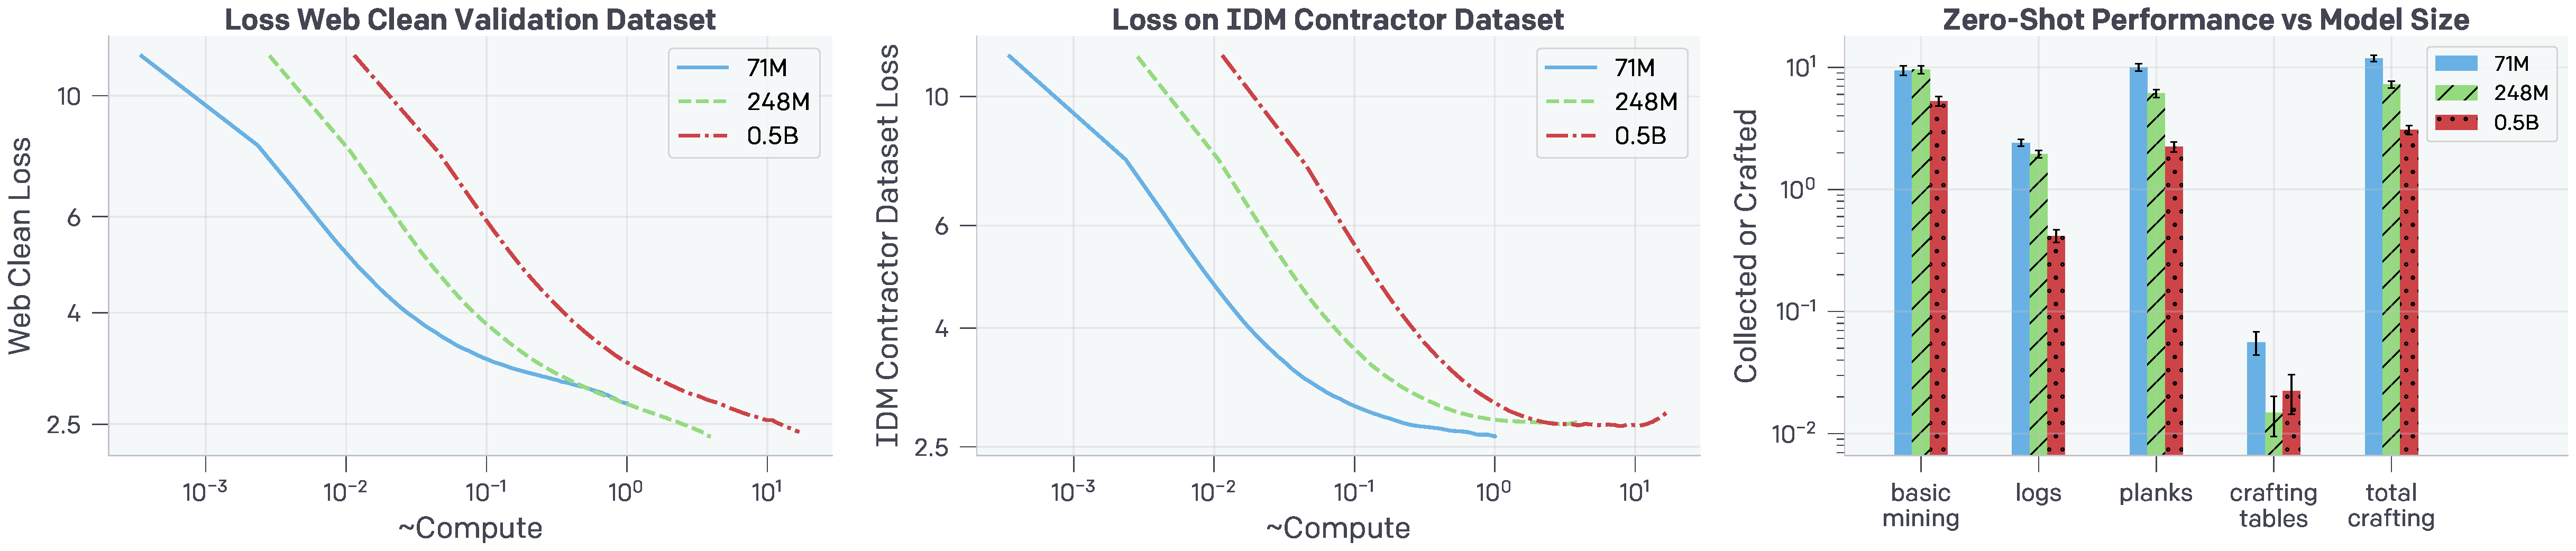
\includegraphics[width=\linewidth]{assets/model_scale_loss_and_zeroshot.pdf} 
\end{subfigure}
\begin{subfigure}{\textwidth}
    \centering
    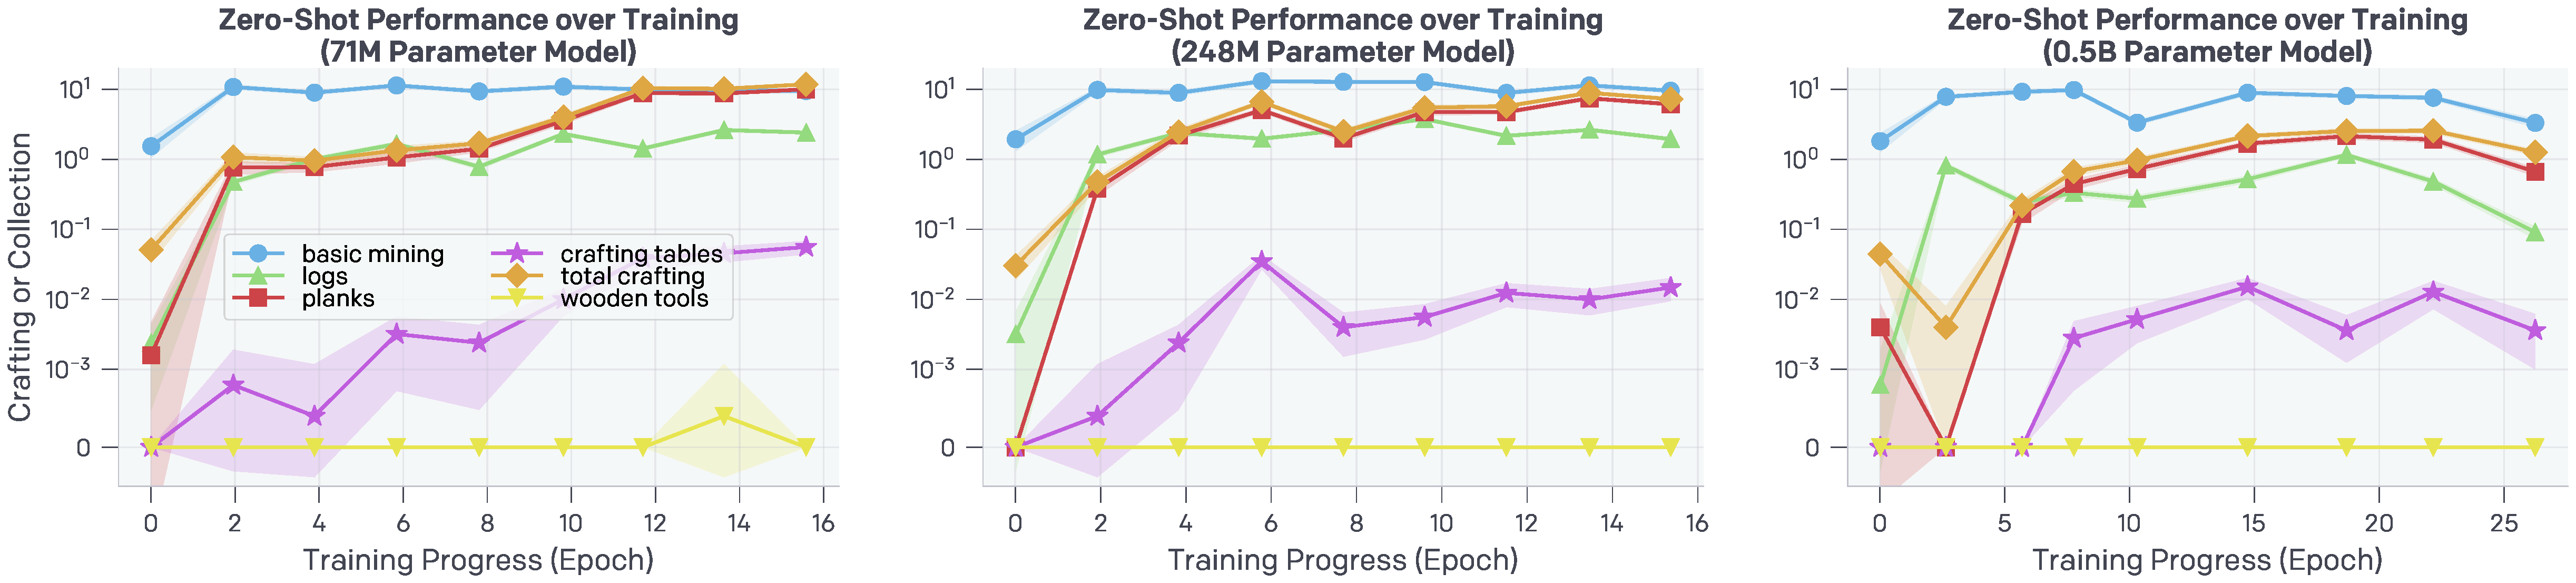
\includegraphics[width=\linewidth]{assets/model_scale_zeroshot_v_version.pdf} 
\end{subfigure}
\caption{
Training and Zero-Shot Performance versus Model Scale. In the first two plots the x-axis is  compute normalized to that used by the 71M parameter model, such that after 15 epochs of training the 71M model has used 1 "compute".  The 248M parameter model and the 71M model are trained on the same amount of data (15 epochs), and the 0.5B parameter model is trained on 30 epochs of data.
\textbf{(Top Left)} Loss on the \texttt{web\_clean} validation dataset.
\textbf{(Top Middle)} Loss on the IDM contractor dataset; note that these models were trained only on \texttt{web\_clean} and not on any contractor data.
\textbf{(Top Right)} Zero-shot environment rollout performance at the end of training.
\textbf{(Bottom)} Zero-shot environment rollout performance over training for the 71M model (bottom left), 248M model (bottom middle), and 0.5B model (bottom right).
}
\label{fig:model_scale_zeroshot}
\end{figure}

In Figure~\ref{fig:model_scale_zeroshot} we show validation loss on \texttt{web\_clean} with IDM pseudo-labels, loss on the contractor dataset used to train the IDM with ground truth labels collected during contractor play, and zero-shot environment performance for the 71M, 248M, and 0.5B models. While larger models have better validation loss on \texttt{web\_clean}, these results do not tell the clear story that the 0.5B model is better than its smaller counterparts. The 71M model has the lowest contractor dataset loss while having the highest \texttt{web\_clean} loss, and it also has the best zero-shot environment performance. In fact, we see that the 71M model even had non-zero wooden tool crafting (Fig.~\ref{fig:model_scale_zeroshot} bottom left). The 248M model also appears to be better at crafting than the 0.5B, and also has lower contractor dataset loss.

\begin{figure}[h]
\centering
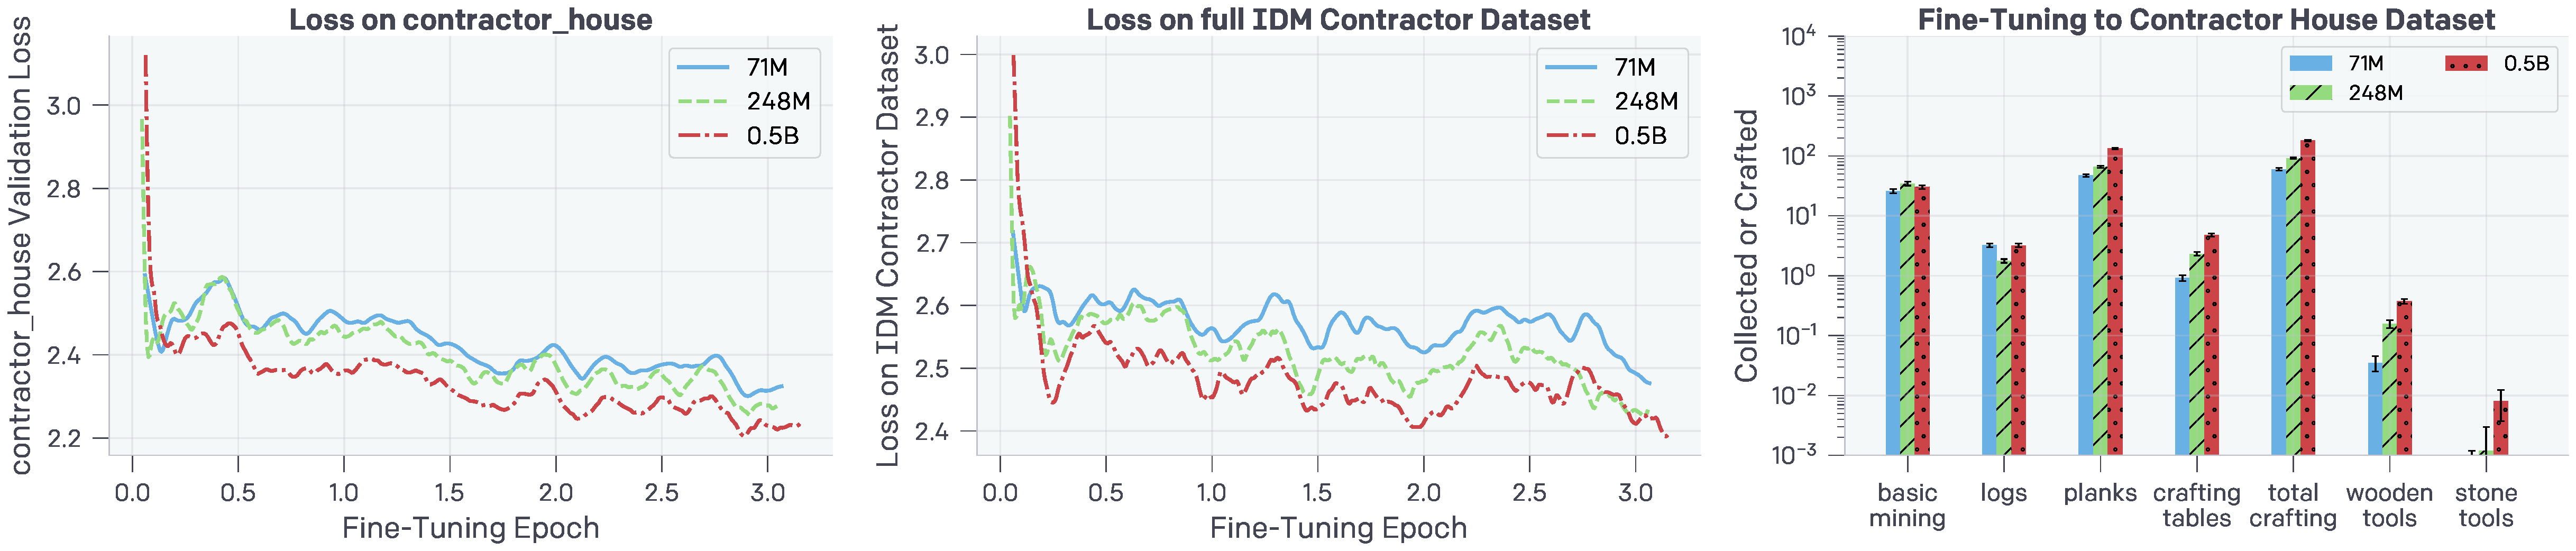
\includegraphics[width=\linewidth]{assets/model_scale_fthouse_loss_and_bar.pdf} 
\caption{
\texttt{contractor\_house} fine-tuning performance versus model size.
\textbf{(Left)} Loss on the \texttt{contractor\_house} holdout validation set.
\textbf{(Middle)} Loss on the full contractor dataset collected to train the IDM; this dataset is disjoint from \texttt{contractor\_house}.
\textbf{(Right)} Environment rollout performance at the end of fine-tuning.
}
\label{fig:model_scale_ft}
\end{figure}

While the zero-shot results suggest smaller models are better, fine-tuning tells another story.
When fine-tuning to \texttt{contractor\_house}, model size rank ordering reverses and now the 0.5B model performs best both in validation loss (Fig.~\ref{fig:model_scale_ft} left) and in environment performance (Fig.~\ref{fig:model_scale_ft} right) followed by the 248M model and then the 71M model.
Environment model rollouts are performed using the same game engine that we use to collect contractor data, which could be visually distinct from videos taken from the web.
It is plausible that the larger models overfocus on the visual peculiarities in web data during pretraining since they have worse contractor data loss (Fig.\ref{fig:model_scale_zeroshot} top middle), and this causes them to perform more poorly in the environment zero-shot. However, we hypothesize that because the \texttt{contractor\_house} dataset we fine-tune to is collected from our game engine, the larger models that are a better overall Minecraft prior (as indicated by lower \texttt{web\_clean} validation loss in Fig.\ref{fig:model_scale_zeroshot} top left) can quickly shift their low level features to perform better on data coming from our game engine, resulting in better environment rollout performance. This hypothesis is further supported by Fig.~\ref{fig:model_scale_ft} (middle) showing loss on the contractor dataset collected for IDM training, which has no overlap with \texttt{contractor\_house}. After just a few steps of fine-tuning to \texttt{contractor\_house}, all models quickly improve in loss on the full IDM contractor dataset, with larger models now performing best. While not conclusive, we believe this investigation provides some intuition for future studies of model scaling for sequential decision making problems.
